\documentclass[letterpaper,12pt]{article}
\usepackage[utf8]{inputenc}

\usepackage{rotating}
\usepackage[top=1in, bottom=1in, left=1in, right=1in]{geometry}
\usepackage{graphicx}
\usepackage[numbers,square,sort&compress]{natbib}
\usepackage{setspace}
\usepackage[cdot,mediumqspace,]{SIunits}
\usepackage{hyperref}
\usepackage{mathtools}
\usepackage{url}
\usepackage{authblk}
\usepackage{placeins}
\usepackage{float}

\onehalfspacing
\title{Astrometric Orbit Determination }
\author{Anita Bahmanyar \qquad Ayushi Singh \qquad Morten Nyborg Stostad \\Department of Astronomy and Astrophysics, University of Toronto}
\affil{\small {Written by: Anita Bahmanyar}}
\affil{\small {anita.bahmanyar@mail.utoronto.ca}}
\affil{\small {Student Number: 998909098}}
%\affil{\small {anita.bahmanyar@mail.utoronto.ca}}
\date{February 3, 2014}

\usepackage{graphicx}

\begin{document}

\maketitle

%Abstract
\begin{abstract}
\label{abstract}
Astrometry is used to measure properties of celestial objects such as their position on the sky, their movement and their velocities. In this experiment, we used a charged coupled device(CCD). The CCD mapped the sky on a 2D plane. Observations were made using the Dunlap Institute Telescope located in New Mexico, United States. The object of interest for this experiment is asteroid named 30 Urania.We measured the plate constants of the CCD using a data from NGC7331 in order to correct for the CCD, since the CCD is not an ideal one. Then we applied these plate constants to the data from 30 Urania over the course of four nights in January 2012 and measured the right ascension and declination of 30 Urania in order to find the orbit of this asteroid. 



\end{abstract}

%Introduction
\section{Introduction}
\label{sec:introduction}
Nowadays, with the advancements of technology, we are able to use computers to do astrom- etry in order to obtain position and motion of celestial objects. We have used the stellar map of NGC7331 taken with DIT and found the centroid points to compared and match them with USNO-B1.0 catalogue in order to find the plate constants of the CCD using least square fitting technique. 


%Experimental Procedure
\section{Experimental Procedure}
\label{sec:experimental procedure}
\subsection{Equipment}
We used the Dunlap Institute Telescope(DIT) which is a 50-cm robotic telescope dedicated to search for optical counterparts of gamma-ray bursts. The telescope was located at New Mexico on Mt. Joy(32:54:10 N +105:31:46 W). The telescope is equipped with a 4096 \begin{math}\times\end{math} 4096 pixel CCD array and the resultant field of view is approximately 36 \begin{math}\times\end{math} 36 arc minutes. Pixel size of this CCD is 9?. This CCD operated in binning mode to collect the data we will be using through this experiment. Binning is useful since it reduces the size of the resultant FITS file and reduces the effect of read-out noise. For 2 \begin{math}\times\end{math} 2 binning the resultant array is 2048 \begin{math}\times\end{math} 2048 pixels.

\section{Analysis}
\label{sec:analysis}
\subsection{CCD Calibration}
In order to have good images from the CCD we need to calibrate them. A good image is one that is dark subtracted and divided by flat frames. Therefore, in order to use the data from the CCD, we subtracted the dark data from the actual data. Dark data was taken with the same exposure time as the actual data while the shutter was closed. Dark current is produced due to the noise in the CCD and it might come from the thermal energy of the electrons; therefore, CCDs are kept in cool places in order to reduce the noise. We also divided the dark subtracted data by the flat frames. Flats are morning and evening twilight sky images that are used to normalize the image. Another factor to consider are the bias frames, which are zero second exposures that provide a measure of digital offset when the signal is zero. Here, the bias is assumed to be zero for this long exposure with DIT.




\section{Asteroid Orbital Elements and Position}
\subsection{Asteroid Position}
The coordinates of astronomical objects are usually measured by the angles right ascension,\begin{math}\alpha \end{math} and declination, \begin{math} \delta \end{math}, in the equatorial system defined by reference stars measured in International Celestial Reference System, taken at epoch 2000. Therefore, the cartesian coordinates are give by equation (...) below.

\begin{equation}
x_{eq}=\cos\alpha \cos\delta, \\ 
y_{eq}=\sin\alpha \cos\delta , \\ 
z_{eq}=\sin\delta
\end{equation}

We can convert the equatorial coordinate to ecliptic coordinate by a transformation along x-axis by the angle \begin{math} \epsilon \end{math} by equation(.....) given below:

\begin{equation}
s=
\begin{pmatrix}
  x \\
  y \\
  z
 \end{pmatrix} 
  =
\begin{pmatrix}
1 & 0 & 0 \\ 
 0 & cos\epsilon & sin\epsilon\\ 
 0 & -sin\epsilon & cos\epsilon
\end{pmatrix}
\begin{pmatrix}
  x_{eq} \\
  y_{eq} \\
  z_{eq}
\end{pmatrix} 
\end{equation}

where \begin{math}\epsilon\end{math} = 23\begin{math} ^{\circ} \end{math}.43929111 for the equinox 2000. s is in the ecliptic Cartesian frame.
In this manner, we are able to calculate the \begin{math}s_{1}\end{math}, \begin{math}s_{2}\end{math} and \begin{math}s_{3}\end{math} vectors and thereafter, we can calculate the first and second derivatives of \begin{math} s_{2} \end{math} vector by equation (...) given below:


% s2 dot equation
\begin{equation}
\dot{s_{2}}=\frac{\tau_{3}(s_{2}-s_{1})}{\tau_{1}(\tau_{1}+\tau_{3})}+\frac{\tau_{1}(s_{3}-s_{2})}{\tau_{1}(\tau_{1}+\tau_{3})}
\end{equation}


% s2 dot dot equation
\begin{equation}
\ddot{s_{2}}=\frac{2(s_{3}-s_{2})}{\tau_{3}(\tau_{1}+\tau_{3})}+\frac{2(s_{2}-s_{1})}{\tau_{1}(\tau_{1}+\tau_{3})}

\end{equation}

The next step is to find the {\bf R} vector. We obtain the components of the {\bf R} vector from the JPL Horizons Ephemeris web interface for the desired date which is 24th, 25th and 26th of January 2012.
The {\bf R} vector components are given in the table (....).

%Table showing right ascension and declination
\FloatBarrier
\begin{table}[h!]
\caption{Date and position of asteroid 30 Urania in the sky} % title of Table
\centering % used for centering table
\begin{tabular}{c c c c } % centered columns (4 columns)
\hline\hline %inserts double horizontal lines
UT Date 2012/01 & Julian Date & Right Ascension(radians) & Declination(radians) \\ [0.5ex] % inserts table
%heading
\hline % inserts single horizontal line
24   &   2455946.68646  & 0.77589496  &  0.33553406  \\
25   &   2455947.69476  & 0.77991461  &  0.33640024  \\
26   &   2455949.73866 &  0.78825718 &   0.33765579  \\ 
27   &   2455950.68528  & 0.79249126 &   0.33851884  \\ [1ex] % [1ex] adds vertical space
\hline %inserts single line
\end{tabular}
\label{table:nonlin} % is used to refer this table in the text
\end{table}
\FloatBarrier




%Table showing the R vector components 
\FloatBarrier
\begin{table}[h!]
\caption{Sun-Earth vector Cartesian components of {\bf R} in ecliptic coordinates [Au]} % title of Table
\centering % used for centering table
\begin{tabular}{c c c } % centered columns (4 columns)
\hline\hline %inserts double horizontal lines
X & Y & Z \\ [0.5ex] % inserts table
%heading
\hline % inserts single horizontal line
-0.4820742567460204  & 0.8578010618775774  &  -2.425231096584922*(10^{(-05)})  \\
-0.4974148410812385  & 0.8490994851434150  &  -2.462584044959891*(10^{(-05)}) \\
-0.5280130493076013  & 0.8306420761670466  &  -2.515673232526080*(10^{(-05)}) \\ 
-0.5419538025371889  & 0.8217251214639645  &  -2.524538626668697*(10^{(-05)})  \\ [1ex] % [1ex] adds vertical space
\hline %inserts single line
\end{tabular}
\label{table:nonlin} % is used to refer this table in the text
\end{table}
\FloatBarrier




We also need to find the magnitude of the R vector for the second data(since the second night is the one we use to find the position of the asteroid as we need three sets of data for figuring out the position). {\bf R} vector magnitude can be calculated by squaring each of the components and taking the square root of their sum.

\begin{equation}
R=\sqrt{R_{x}^2+R_{y}^2+R_{z}^2}
\end{equation}


We now have all the values we need and should be able to calculate \begin{math} \rho \end{math} value by the equation (...):

\begin{equation}
\rho=k^2(\frac{1}{R^3}-\frac{1}{r^3})\frac{\dot{{\bf s}}.({\bf R}\times{\bf s})}{\dot{{\bf s}}.(\ddot{{\bf s}}\times{\bf s})}
\end{equation}

We do not have the value or r explicitly yet; however, we can guess an initial r value and write a for loop to calculate \begin{math} \rho \end{math} until it converges using the new values for r. This part of the code I used can be found in the appendix.(....)


After finding the \begin{math} \rho \end{math} value, we can calculate the r value by equation (....):

\begin{equation}
r^2=\rho ^2 + R^2 + 2\rho {\bf R}. {\bf s}
\end{equation}

Note that this r is different from the one we just guessed in equation (.....). 
We can also calculate derivative of \begin{math} \rho \end{math} using equation (....) :
\begin{equation}
\dot{\rho}=\frac{k^2}{2}(\frac{1}{{\bf R}^3}-\frac{1}{r^3})\frac{\ddot{s}.({\bf R}\times {\bf s})}{\ddot{{\bf s}}.({\bf \dot{s}}\times {\bf s})}
\end{equation}

We can now calculate the position vector of the asteroid with respect to sun using simple vector addition:

\begin{equation}
{\bf r}= {\bf R}+r{\bf s}
\end{equation}
We may also find the derivative of the {\bf R} vector using the same way we found the derivative of the vector {\bf s}, which can be written as equation (...):

\begin{equation}
\dot{{\bf R_{2}}}=\frac{\tau_{3}({\bf R_{2}}-{\bf R_{1}})}{\tau_{1}(\tau_{1}+\tau_{3})}+\frac{\tau_{1}({\bf R_{3}}-{\bf R_{2}})}{\tau_{1}(\tau_{1}+\tau_{3})}
\end{equation}

In order to calculate the velocity of the asteroid relative to the sun we need to find the derivative of the {\bf r} vector we found in equation (...) and employ equation (....):

\begin{equation}
{\bf \dot{r}}={\bf \dot{R}} +\rho{\dot{\bf s}} + \dot{\rho} {\bf s}
\end{equation}


\subsection{Orbital Elements}
We can now use the values we got from previous section to find the orbital elements of 30 Urania using Laplace's method. Since we know the magnitude of the radius vector, r, and the total velocity, V, we can compute the semimajor axis by eqaution (....):

\begin{equation}
a=\frac{k^2r}{2k^2-rV^2}
\end{equation}

Then we can compute the {\bf h} vector components by the cross product of the {\bf r} and {\bf \dot{r}} vectors:
\begin{equation}
{\bf h}= {\bf r} \times {\bf \dot{r}}
\end{equation}
Using the {\bf h} vector components, we can compute \begin{math} \Omega \end{math} and i by equations (....) and (...) respectively:

% Omega orbital element
\begin{equation}
\tan \Omega = \frac{-h_{x}}{h_{y}}
\end{equation}

% i orbital element
\begin{equation}
\cos i = \frac{h_{z}}{h}
\end{equation}

In order to find the eccentricity, we use equation (...) given below:

% eccentricity orbital element
\begin{equation}
e=\sqrt{1-(\frac{h^2}{ak^2})}
\end{equation}

In order to compute the last two Keplerian orbital elements,-the argument of perihelion,\begin{math} \omega \end{math}, and the epoch of perihelion, \begin{math} \tau \end{math}, we need to calculate the eccentric and true anomalies. Equation (....) and (...) give the eccentric and true anomalies, respectively.

% eccentric anomaly orbital element
\begin{equation}
\cos E = \frac{a-r}{ae}
\end{equation}

% true anomaly orbital element
\begin{equation}
\cos (v+\omega) = \frac{x \cos \Omega + y \sin \Omega}{r} 
\end{equation}

%\FloatBarrier
%\begin{figure}[h!]
%\centering
%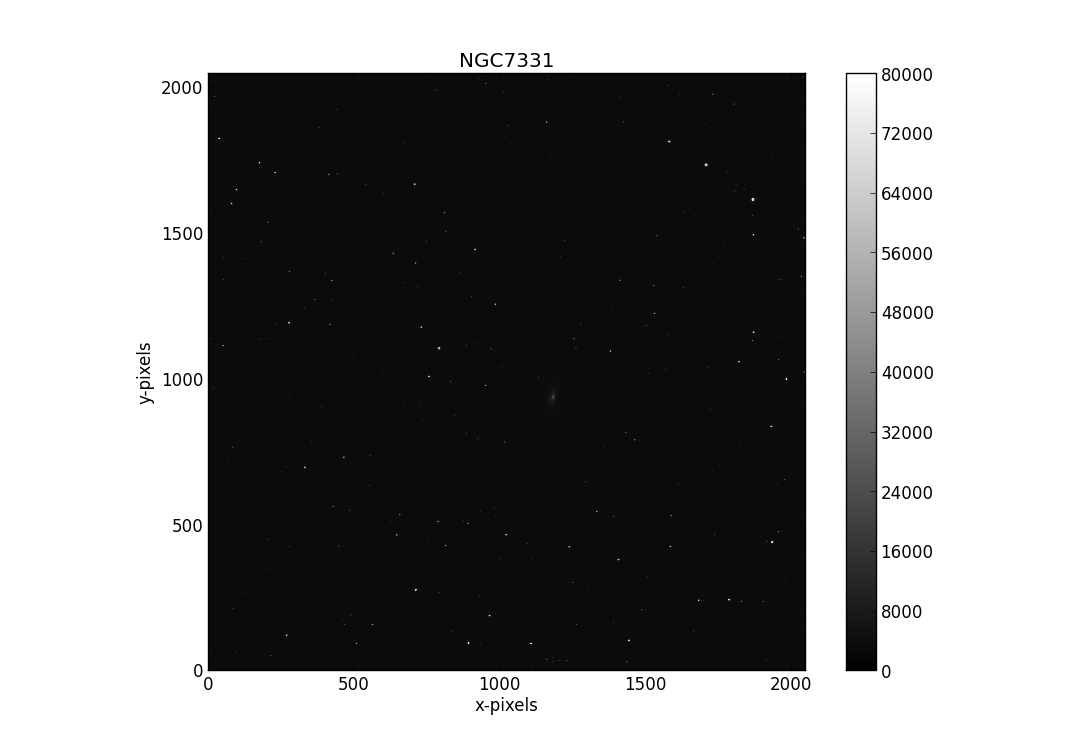
\includegraphics[scale=0.6]{ngc7331.png}
%\caption{This figure shows the NGC7331. The colour bar shows the intensity of the objects with black having zero intensity. This image is dark subtracted and divided by flat in order to be normalized.}
%\end{figure}
%\FloatBarrier

\end{document}


